%%%%%%%%%%%%%%%%%%%%%%%%%%%%%%%%%%%%%%%%%%%%%%%%%%%%%%%%%%%%%%%%%%%%%%%%%%%

\documentclass[letterpaper, 10 pt, conference]{ieeeconf}  % Comment this line out if you need a4paper

%\documentclass[a4paper, 10pt, conference]{ieeeconf}      % Use this line for a4 paper

\IEEEoverridecommandlockouts % This command is only needed if you want to use the \thanks command

\overrideIEEEmargins % Needed to meet printer requirements.

% See the \addtolength command later in the file to balance the column lengths
% on the last page of the document

\usepackage[latin1]{inputenc}
\usepackage{pgfplots}
\usepackage{tikzscale}
\usepackage{epstopdf}
\usepackage{amsmath}
%\usepackage{amsthm}
\usepackage{amsfonts}
\usepackage{amssymb}
\usepackage{mathtools}
\usepackage{graphicx}
\usepackage{color}
\usepackage{subfig}
\usetikzlibrary{plotmarks}
%\usepackage{hyperref}

% theorem environment
\newtheorem{prop}{Proposition}[section]
\newtheorem{theorem}{Theorem}[section]
\newtheorem{prop2}{Proposition}
\newtheorem{lem}{Lemma}
\newtheorem{ex}{Example}

% For algorithms
\usepackage{algorithm}
\usepackage{algorithmic}

% custom commands
\newcommand{\boldvec}[1]{\boldsymbol{\mathrm{#1}}}
\let\vec\boldvec
\newcommand\at[2]{\left.#1\right|_{#2}} % the at differential sign
\newcommand\scalemath[2]{\scalebox{#1}{\mbox{\ensuremath{\displaystyle #2}}}} % scaling matrices
\DeclareMathOperator{\vect}{vec}

%% custom macros
\newcommand{\todo}{\textcolor{red}{TODO}} % TODO!
\newcommand{\kin}{\mathcal{T}} % used to denote inverse kinematics
\newcommand{\invKin}{\mathcal{T}^{-1}} % used to denote inverse kinematics

\newcommand{\joint}{\vec{q}} % used to denote robot state in joint space
\newcommand{\state}{\vec{y}} % denotes the generalized coordinates - joint space and velocity coordinates
\newcommand{\error}{\vec{e}} % difference between state and reference
\newcommand{\traj}{\vec{r}} % used to denote the points on the trajectory to be tracked

\newcommand{\dist}{\vec{\epsilon}} % denotes the disturbances acting on the rigid body dynamics
\newcommand{\linDist}{\vec{d}} % denotes the disturbances on the LTV model

\newcommand{\sysInput}{\vec{u}} % used to denote the system inputs
\newcommand{\linInput}{\tilde{\sysInput}} % denotes the LTV inputs
\newcommand{\trjInput}{\sysInput_{\mathrm{IDM}}} % denotes the inputs on the trajectory (calculated using IDM)
\newcommand{\ilcInput}{\sysInput_{\mathrm{ILC}}}


% % % % DMP terminology % % % %
\newcommand{\dmp}{s} % used to denote the dmp trajectory states
\newcommand{\goal}{g} % goal state
\newcommand{\force}{\mathit{f}} % forcing term of the dmps
\newcommand{\phase}{\phi} % phase of the dmp
\newcommand{\weights}{w} % weights of the dmp
\newcommand{\basis}{\Psi} % basis functions of the dmp as a matrix
\newcommand{\amp}{A} %amplitude of the rhythmic dmp
\newcommand{\basisHeight}{h} % basis fnc parameters
\newcommand{\basisCenter}{c}

% % % % ILC terminology % % % %
\newcommand{\qmatrix}{\vec{\Gamma}} % denotes the filtering qmatrix term of Bristow et al.
\newcommand{\lmatrix}{\vec{L}} % denotes the learning matrix of Bristow et al.

\newcommand{\dynamics}{\vec{f}}
\newcommand{\dynamicsNominal}{\dynamics_{\mathrm{nom}}}
\newcommand{\policy}{\vec{\pi}}
\newcommand{\ValueFunction}{J}
\newcommand{\episode}{k} % used for episode number

\newcommand{\totalTime}{T} % total time duration 
\newcommand{\numSteps}{N} % total number of time steps
\newcommand{\numepisode}{K} % total number of episodes

\newcommand{\threshold}{\epsilon}
\newcommand{\alg}{\emph{gILC}}
\newcommand{\dataset}{E}

% Set the paths where all figures are taken from:
\graphicspath{{Pictures/}}
\mathtoolsset{showonlyrefs} 
\newcommand{\includesvg}[1]{%
% \executeiffilenewer{#1.svg}{#1.pdf}%
% {inkscape -z -D --file=#1.svg %
% --export-pdf=#1.pdf --export-latex}%
 \input{#1.pdf_tex}%
}

%\addtolength{\topmargin}{50pt}
\title{\LARGE \bf
Optimizing Robot Striking Movement Primitives with Iterative Learning Control
}

\author{Okan Ko\c c$^{1}$, Guilherme Maeda$^{2}$, Gerhard Neumann${^2}$, Jan Peters$^{1,2}$% <-this % stops a space 
\\
{\tt\small \{okan.koc, jan.peters\}@tuebingen.mpg.de}%
\thanks{$^{1}$Max Planck Institute for Intelligent Systems,
        Spemannstr. 38, 72076 Tuebingen, Germany}
\thanks{$^{2}$Technische Universitaet Darmstadt, FG Intelligente Autonome Systeme
        Hochschulstr. 10, 64289 Darmstadt, Germany}
}

\begin{document}

\maketitle
\thispagestyle{empty}
\pagestyle{empty}

%%%%%%%%%%%%%%%%%%%%%%%%%%%%%%%%%%%%%%%%%%%%%%%%%%%%%%%%%%%%%%%%%%%%%%%%%%%
\begin{abstract}

Highly dynamic tasks that require large accelerations and precise tracking usually rely on precise models and/or high gain feedback. While
movement primitives allow for the efficient representation of such tasks, the optimization of the required motor commands for systems with inaccurate dynamic models remains an open problem.
%Complex robot motor skills can be represented efficiently with a sequence of movement primitives. However, in order to perform the task effectively, the robot needs to be able to execute the corresponding primitives well. 
To achieve accurate tracking for such tasks, we investigate two related Iterative Learning Control update laws and present a variant suited for optimizing hitting movement primitives. The resulting algorithm generalizes well to different initial conditions and naturally addresses striking movements where reaching specific velocities at certain positions is crucial. We evaluate the performance of our approach in a simulated putting task as well as in 
%a real 
robotic table tennis,
% platform
where we show how the striking performance of a seven degree of freedom anthropomorphic arm can be optimized. Our final implemented algorithm compares favorably with two state-of-the-art approaches.

\end{abstract}

%%%%%%%%%%%%%%%%%%%%%%%%%%%%%%%%%%%%%%%%%%%%%%%%%%%%%%%%%%%%%%%%%%%%%%%%%%%

\section{INTRODUCTION}\label{introduction}

% fill missing citations

Most reaching tasks in control and robotics can be phrased as \emph{tracking} problems, where the dynamical system needs to follow a certain predefined trajectory in order to reach the goal state. Robotic table tennis in particular~\cite{Muelling13} consists of planning, generating and executing a series of such (episodic) single stroke trajectories. These trajectories need to be followed very closely with motor commands in practice, in order to return the ball to the goal position. 

% maybe cite Jens' review paper
There have been many attempts in the reinforcement learning (RL)~\cite{Sutton98} and control literature to learn robotic tasks directly. Value function based methods take advantage of duality to solve the Bellman's equation but suffer from the initial bias or representation in estimating the value function and do not scale well to high dimensions. Policy search based RL methods (e.g.,~\cite{Kober08}, \cite{Peter10}, \cite{Theodorou10}, \cite{Deisenroth11}) directly solve the Bellman's equation in a parameterized policy space and can be more effective in practice~\cite{Kober13}. 

Dynamic Movement Primitives (DMP) are a kind of kinematic policy representation that leverages the dynamical systems approach to modify the spring dynamics with a forcing term that enables it to mimic an executed trajectory. They include an internal phase or clock that ensures the convergence of the movement primitive to a goal state~\cite{Ijspeert13}, \cite{Schaal07}. DMPs do not suffer from the curse of dimensionality as the number of parameters (weights) grow linearly with dimension. However, approximation and control errors in robotic platforms make the application of DMPs less useful in practice. Small changes to DMPs can often make them more useful.

Motor primitives can be modulated in different ways to adapt to unforeseen events or to ensure the optimal execution of required tasks. They work particularly well with episodic policy search methods that modify the weights of the forcing term based on the rewards received in every episode. By adapting the DMP that was initialized with imitation learning e.g., with kinesthetic teach-in~\cite{Muelling13}, RL approaches are able to achieve complex robotic tasks, such as ball-in-a-cup~\cite{Kober09}. However model-free methods (e.g., \cite{Kober08}, \cite{Peter10}) require many iterations to converge, whereas more data-efficient approaches such as~\cite{Deisenroth11} suffer from computational runtime difficulties and cannot be implemented in real-time robotics tasks. Optimality of the converged policy cannot be guaranteed by these methods.
% maybe mention reference trajectory?
% model-free ? PILCO claims to be 'model-based', yet it learns from scratch. It only 'learns' a model, but it is unbiased.

% inaccurate ?
Inspired by the successes (and failures) of these previous approaches, the research question that we tackle in this article consists of the following:
%
\begin{itemize}
\item How can we execute optimally hitting movement primitives either in table tennis or a similar reaching task e.g., putting in golf.
%
\item More specifically, when we have modelling inaccuracies, how should we modify a DMP $\dmp(t)$ such that the robot executes a desired hitting motion?
\end{itemize}
%
\begin{figure}[b!]
\center
\includegraphics[scale=0.4]{robot1.png}			
\caption{Robotic table tennis setup with the ball-launcher throwing balls to the robot. In order to hit the ball to a desired position on the opponent's court, we give the robot reference trajectories that facilitate the right striking motion. We can teach the robot such trajectories via kinesthetic teach-in.}
\label{robot}
\end{figure}
%
% maybe include P. Abbeel's work on inaccurate models
\noindent We believe that learning in robotics tasks can be performed much more efficiently by taking advantage of existing imperfect models and reference trajectories. % optimality issues can be alleviated with given reference trajectories. 

Iterative Learning Control (ILC) is a fundamental approach in control theory developed to track (time-varying) reference trajectories. It has been used successfully to follow trajectories under unknown repeating disturbances and model mismatch \cite{Bristow06}. In ILC, control inputs are adjusted at each episode in a feedforward fashion. The goal is to drive the deviations from the trajectory to zero. 
% or equivalently references

In this article, we combine Iterative Learning Control with movement primitives by using ILC as a learning method to adapt the weights of the DMPs. This way we ensure a safe, reliant and robust way to track reference trajectories, with important applications in optimally hitting and striking motions. As opposed to model-free policy search approaches, we make full use of the known, albeit inexact, robot dynamics and inverse dynamics models, which helps us to quickly achieve the desired performance requirements. We validate the performance of the approach in two hitting tasks, and compare with existing episodic-RL approaches.
% nominal model instead of known, albeit inexact?

Our contributions can be summarized as follows: we form a link between the ILC literature and the movement primitives by systematically formulating an iterative update of the DMP weights. We form a coherent learning framework and present new motor primitive update laws. These are studied in detail and the implemented ILC algorithm~$\alg$ is shown to perform better than existing RL approaches in two hitting tasks, putting and table tennis.

In Section~\ref{relatedWork} we mention related work, especially the state of the art approaches in hitting and reaching tasks. In Section~\ref{problemStatement} we state the problem and introduce motor primitive update laws, relating them to the existing optimization-based ILC approaches. We formulate one of these update laws, called $\alg$, in algorithmic form in Section~\ref{algorithm}. In Section~\ref{experiments} we evaluate $\alg$ in two robotic reaching tasks: putting motion in golf and the striking motions in table tennis. We show that the method outperforms the state-of-the-art RL-based approaches \emph{REPS} and \emph{PI$^{2}$}. Finally in Section~\ref{conclusion} we discuss the strengths and weaknesses of our method and conclude with brief mentions of promising future research directions.

\subsection{Related Work}\label{relatedWork}

% mention the ILC paper of Peter Abbeel
Dynamic movement primitives belong to the class of movement primitives~\cite{Flash85}. Movement primitives are a kinematics-based approach to keep the learning tasks in high-dimensional tasks, such as in humonoid robotics, tractable. Like the options framework in Markov Decision Processes, they aim at reducing the curse of dimensionality in complex human-like robotics tasks. The first dynamical systems based formulation of movement primitives appeared in~\cite{Ijspeert02}. A good review with alternative and variant formulations is given in~\cite{Ijspeert13}.

% Policy search methods
One of the first examples of policy search based methods that modify the parameters of movement primitives is the \emph{POWER} algorithm~\cite{Kober08}. \emph{PI$^{2}$} algorithm has a very similar implementation in~\cite{Theodorou10} and episodic-\emph{REPS}~\cite{Peter10} is actually equivalent to \emph{POWER}.

Iterative Learning Control started out in the 1980s with the work of Arimoto et al.~\cite{Arimoto84} as one of the first to define the genre with the PD-type update law. See~\cite{Bristow06} and \cite{Moore99} for reviews. Monotonic convergence and stability guarantees are of central importance for the practical usefulness of ILC algorithms. They are shown for example in~\cite{Bristow06}, \cite{Norrloef02}, \cite{Longman2000}.

% ILC work - mention Angela's work
As an example of a more sophisticated method than the PD-type update laws, Schoellig et al.~\cite{Schoellig12} applied a Kalman-filter based convex optimization rule in the framework of ILC and showed its performance in quadrocopter flight. An EM-based update law was given in~\cite{Berg10} where an impressive application of ILC to a robotic surgical task was presented.
% This work however lacks any guarantees of monotonic convergence

% DMPs using Iterative Learning Control
DMPs have been also combined in a bimanual robotics task with ILC~\cite{Gams13} where force feedback is used to enable compliant interaction with objects in an unknown environment. ILC is here used to learn a coupling term between the two arm trajectories. To the best of our knowledge, ILC has not been used so far to modify the weights of the movement primitives.
% used to modulate the DMP and learn ...

\subsection{Problem Statement}\label{problemStatement}

The goal in trajectory tracking is to track a given reference $\traj(t), \ 0 \leq t \leq T \ $, in state space $\state \in S \subset \mathbb{R}^{n}$ by applying the control inputs $\sysInput(t)$. The reference trajectory in our case enables the \emph{optimal} execution of hitting and striking motions, e.g., forehand and backhand strikes in (table) tennis. We assume that such optimal trajectories are available to us, either through kinesthetic teach-in or computed recursively.
% talk about feasibility.
% reference needed? Dynamic programming?

% subsubsection entitled 'modelling assumptions'?
% talk of model-free regression update of DMP there maybe?
Consider the nonlinear robot dynamics of the form
%
\begin{equation}
\begin{aligned}
\ddot{\joint} &= \dynamics(\joint,\dot{\joint},\sysInput), \\
\ddot{\joint} &= \vec{M}^{-1}(\joint)\{ \vec{\tau}(\sysInput) - \vec{C}(\joint,\dot{\joint})\dot{\joint} - \vec{G}(\joint)\} + \dist(\joint,\dot{\joint}),\\
\end{aligned}
\label{dynamics}
\end{equation}
%
\noindent where on the right hand side are the terms due to the rigid body dynamics model and $\dist(\joint,\dot{\joint})$ are the (unmodeled) disturbances that act on the robot, such as viscous friction, stiction, etc. This system can be linearized around a given joint space trajectory $\traj(t), \ 0 \leq t \leq T$ with nominal inputs $\trjInput(t)$ calculated using the inverse dynamics model. We then obtain the following linear time varying (LTV) representation
%
\begin{equation}
\begin{aligned}
\dot{\error} = \vec{A}^{c}(t)\error(t) + \vec{B}^{c}(t)\linInput(t) + \linDist(t,\sysInput),
\end{aligned}
\label{LTV}
\end{equation}
%
\noindent where the state error is denoted as $\error(t) = \state(t) - \traj(t)$, the joint angles and velocities are $\state = [\joint,\dot{\joint}]^{\mathrm{T}}$, $\linInput(t) = \sysInput(t) - \trjInput(t)$ and the continuous time varying matrices are
%
\begin{equation}
\begin{aligned}
\vec{A}^{c}(t) &= \at{\frac{\partial{\dynamics}}{\partial{\state}}}{(\traj(t),\trjInput(t))}, \\
\vec{B}^{c}(t) &= \at{\frac{\partial{\dynamics}}{\partial{\sysInput}}}{(\traj(t),\trjInput(t))}.
\end{aligned}
\label{LTVmatrices}
\end{equation}
%
% what about estimation errors, i.e. sensor errors ...
\noindent In the error dynamics \eqref{LTV} the additional term $\linDist(t,\sysInput)$ accounts for the disturbances and the effects of the linearization. We can discretize (\ref{LTV}-\ref{LTVmatrices}) with step size $\delta$, $N = T/\delta$ and step index $j = 1, \ldots, N$ to get the following discrete linear system
%
\begin{equation}
\begin{aligned}
\error_{j+1} = \vec{A}_j\error_j + \vec{B}_j\linInput_j + \linDist_j(\sysInput_1, \ldots, \sysInput_j),
\end{aligned}
\label{discreteLTV}
\end{equation}
%
\noindent where the matrices $\vec{A}, \vec{B}$ are the discretizations of \eqref{LTVmatrices}. Conventional ILC algorithms learn to compensate for the errors by iterating the control inputs $\sysInput$ with an update law.
\section{Iterative Learning Control with Movement Primitives}\label{method}

In a complex task such as robot table tennis, one often needs to consider an extension of the standard trajectory tracking task. Based on the varying initial positions and velocities of the robot arm and the trajectory of the incoming ball, in each table tennis stroke the robot arm needs to track different trajectories that start from different initial conditions and end with different goal states of the arm. Moreover these trajectories need to be scaled in time to intercept the ball. Dynamic Movement Primitives (DMP) are especially useful for representing such a variety of movement patterns.
% reference needed? revise.

%Sometimes for safety reasons, for instance when interacting with external objects or under unforeseen perturbations \cite{Schaal07}, a \emph{low-gain} feedback law operating on the inputs may be fine-tuned to be compliant. As another practical restriction, one may not even be allowed to modify the low-level controller of the industrial robot \cite{Longman2000}. In such cases, it is not possible to modify the input signals $\sysInput$ directly. Instead one can modify the reference trajectories that are provided to the low-level controllers. It can be shown that this is an equivalent approach to modifying the feedforward control inputs \cite{Bristow06}.

Based on these considerations, in this paper we focus on learning to track DMPs $\dmp(t) = [\joint_{\text{des}}(t),\dot{\joint}_{\text{des}}(t)]^{\mathrm{T}}$. An initial DMP might be constructed out of a given demonstration or an optimal reference trajectory $\traj(t)$ using regression techniques \cite{Ijspeert13}. Representing a reference trajectory with movement primitives has some benefits: nonsmooth parts of the trajectory can be filtered, the evolution of desired states can be coupled with errors to ensure safety, time and scaling invariance of the differential equations can be used to adapt the trajectory to task changes in time as well as in space. %Robustness to initial joint position and velocity changes 

\subsection{Movement Primitive Formulation}
The dynamic movement primitive equations~\cite{Kober08} can be written as a weakly nonlinear system 
%
\begin{equation}
\begin{aligned}
\dot{\dmp} &= \begin{bmatrix}
   \dot{\dmp}_1 \\
   \dot{\dmp}_2
 \end{bmatrix} = \tau \begin{bmatrix}
     \dmp_2  \\
     \alpha_{g} (\beta_{g}(\goal - \dmp_1) - \dmp_2) +  \vec{\phi}(\phase)\weights
  \end{bmatrix}
\label{dmp},
\end{aligned}
\end{equation}
%
\noindent where the phase $\phase$ evolves according to
%
\begin{equation}
\dot{\phase} = -\tau\alpha_{\phase}\phase.
\label{phase}
\end{equation}
%
\noindent The constants $\tau$ and $\alpha_{\phase}$ determine the scaling and settling time respectively. 

The dynamical system \eqref{dmp} describes the motion of each of the desired joint states along a particular path in joint space. The forcing terms $\force = \vec{\phi}(\phase)\weights$ determine this path by warping the motion of the spring dynamics. The weights $\weights$ are obtained from regression using demonstration data. The spring constants $\alpha_{g}$ and $\beta_{g}$ ensure that starting from any initial position and velocity $\dmp_0$ the DMP converges to the goal state $\goal := \dmp_T = \traj_T$ and are usually chosen such that the dynamical system is critically damped.

% mention Jens' and Katharina's extension for hitting DMPs with desired velocity

% a figure showing convergence from different starting conditions needed here

\subsection{Derivation of ILC Updates}

Most ILC update laws can be put in the following form

\begin{equation}
\begin{aligned}
\sysInput_{k+1} = \qmatrix(\sysInput_{k} - \lmatrix\error_{k}).
\end{aligned}
\label{ILCupdateForm}
\end{equation}

\noindent Model based ILC can be cast in this form by stacking the model matrices in \eqref{discreteLTV} together to get the following lifted-vector representation \cite{Bristow06}, \cite{Schoellig12}

\begin{equation}
\begin{aligned}
\error_L &= \vec{F}\sysInput_L + \linDist_L, \\
\end{aligned}
\label{liftedLTV}
\end{equation}

\noindent where the submatrices of $\vec{F}$ are

\begin{equation*}
\begin{aligned}
\vec{F}_{(i,j)} &= \left \{
\begin{array}{cc}
\vec{A}_{i-1}\ldots \vec{A}_j \vec{B}_{j-1}, & j < i, \\ 
\vec{B}_{j-1}, & j = i, \\
\vec{0}, & j > i. 
\end{array} \right.
\end{aligned}
\end{equation*}

\noindent Using this \emph{input-to-output matrix} $\vec{F}$ we can analyze the effects of the feedforward inputs $\sysInput_L = [\linInput_1, \linInput_2, \ldots, \linInput_{\numSteps}]^{\mathrm{T}}$ on the errors $\error_L = [\error(1),\error(2),\ldots,\error(\numSteps)]^{\mathrm{T}}$ and compensate for the disturbances $\linDist_L$ with ILC.

%\noindent If the disturbances are repeating every iteration, i.e. $\frac{\partial{\linDist_L}}{\partial{\sysInput_L}} = 0$, using \eqref{liftedLTV},

\subsubsection{Lagrange form} The quadratic cost functional as the optimality criterion

\begin{equation}
\begin{aligned}
\ValueFunction(\state_0) &= \int_{0}^{T} \error^{\mathrm{T}}\vec{Q}\error + \linInput^{\mathrm{T}}\vec{R}\linInput \ \mathrm{d}t + \error_{T}^{\mathrm{T}}\vec{Q}_{T}\error_{T},
\end{aligned}
\label{cost}
\end{equation}

\noindent can be equally discretized and stacked in lifted vector form

\begin{equation}
\begin{aligned}
\ValueFunction_L &= \error_L^{\mathrm{T}}\vec{Q}_L\error_L + \sysInput_L^{\mathrm{T}}\vec{R}_L\sysInput_L,
\end{aligned}
\label{costFunctional}
\end{equation}

\noindent where $\vec{Q}_L \in \mathbb{R}^{2Nn \times 2Nn}$ (similarly for $\vec{R}_L$) is of the following form
%
\begin{equation*}
\begin{aligned}
 \vec{Q}_L &= 
 \begin{bmatrix}
  \vec{Q} & \vec{0} & \cdots & \vec{0} \\
  \vec{0} & \vec{Q} & \cdots & \vec{0} \\
  \vdots  & \vdots  & \ddots & \vdots  \\
  \vec{0} & \vec{0} & \cdots & \vec{Q}_T
 \end{bmatrix}.
\end{aligned}
\end{equation*}

\noindent Using Gauss-Newton we can optimize iteratively for $\sysInput_L$

\begin{equation}
\begin{aligned}
\sysInput_{k+1} &= \sysInput_k - \Big(\frac{\partial^{2}\ValueFunction_L}{\partial\sysInput^{2}_L}\Big)^{-1}\at{\frac{\partial{\ValueFunction_L}}{\partial{\sysInput_L}}}{\sysInput_k} \\
\frac{\partial^{2}\ValueFunction_L}{\partial\sysInput^{2}_L} &= \frac{\partial}{\partial\sysInput_L}\{F^{\mathrm{T}}Q_L\error_L\} = F^{\mathrm{T}}Q_LF \\
\sysInput_{k+1} &= \sysInput_k - \beta_kF^{\dagger}\error_k
\end{aligned}
\label{ILCnewtonsMethod}
\end{equation}

\noindent ILC update law can be related to Newton's method if we consider the Hessian of the cost functional \eqref{cost2}
%
\begin{equation}
\begin{aligned}
\weights_{k+1} &= \weights_k - \beta_k\Big(\frac{\partial^{2}\ValueFunction}{\partial\weights^{2}}\Big)^{-1}\at{\frac{\partial{\ValueFunction}}{\partial{\weights}}}{\weights_k}, \\
\frac{\partial^{2}\ValueFunction}{\partial\weights^{2}} &= \frac{\partial}{\partial\weights}\{\vec{F}_{w}^{\mathrm{T}}\vec{Q}_L\error_L + \vec{R}_w\weights\} = \vec{F}_{w}^{\mathrm{T}}\vec{Q}_L\vec{F}_{w} + \vec{R}_{\weights}, \\
\weights_{k+1} &= \qmatrix\weights_k - \beta_k(\vec{F}_{w}^{\mathrm{T}}\vec{Q}_L\vec{F}_{w} + \vec{R}_{w})^{-1}\vec{F}_{w}^{\mathrm{T}}\vec{Q}_L\error_k,
\end{aligned}
\label{ILCWeightsNewtonsMethod}
\end{equation}
%
\noindent where the filtering matrix is $\qmatrix = \beta_k(\vec{F}_{w}^{\mathrm{T}}\vec{Q}_L\vec{F}_{w} + \vec{R}_{w})^{-1}\vec{R}_{w}$. 

Note the connection of \eqref{ILCWeightsNewtonsMethod} to plant inversion methods~\cite{Bristow06}: taking $\vec{Q}_L = \vec{I}, \vec{R}_{w} = \vec{0}, \beta = 1,$ \eqref{ILCWeightsNewtonsMethod} becomes
%
\begin{equation}
\begin{aligned}
\weights_{k+1} &= \weights_k - \vec{F}_{w}^{\dagger}\error_k.
\end{aligned}
\label{ILCPlantInversion}
\end{equation}
%
% However this can be very unstable in practice, especially in nonminimum phase systems. Having a small, but nonzero weighting matrix R makes it much more stable.
%
\noindent Notice also the connection of \eqref{ILCRegression} with the online regression methods performed on the DMP weights \cite{Ijspeert13}. We can rewrite \eqref{ILCWeightsNewtonsMethod} as
%
\begin{equation}
\begin{aligned}
\weights_{k+1} &= \weights_k - \beta_k(\vec{\Psi}^{\mathrm{T}}\vec{W}\vec{\Psi} + \vec{R}_{w})^{-1}\vec{\Psi}^{\mathrm{T}}\vec{W}\error_k, \\
\vec{\Psi} &= \begin{bmatrix}
  \basis_1^{T} & \basis_2^{T} & \ldots & \basis_N^{T}
 \end{bmatrix}^{T}.
\end{aligned}
\label{ILCRegression}
\end{equation}
%
%
% online regression methods? are they discussed in the given reference?
In model-free approaches the weighting matrix $\vec{W}(t)$ is taken as the identity matrix. In our case the model-based assumptions of our approach appear in the form of a nondiagonal covariance matrix. We perform generalized least-squares regression by taking advantage of the linearized model in~\eqref{fullTransition} to form the right correlations between states. Compared with the \emph{credit-assignment} issues of RL algorithms, we see that ILC, equipped with our linearized models, offers us a more principled way to assign errors to the weights of the movement primitives.

\subsubsection{Mayer form}

\subsection{Iterative Learning Control for Movement Primitives}\label{ilcOnDMP} 

For the linearization of the robot dynamics \eqref{dynamics} under a given linear feedback law $\linInput(t) = -\vec{K}(t)(\state - \dmp)$ we consider the addition of the movement primitive dynamics to \eqref{LTV} 
%
\begin{equation}
\begin{aligned}
\dot{\fullvec} &= \vec{A}_{\fullvec}\fullvec(t) + \vec{B}_{\fullvec} \weights + \linDist(t,\weights),
\label{fullTransition}
\end{aligned}
\end{equation}
%
\noindent where for the enlarged vector $\fullvec = [\error,\dmp]^{\mathrm{T}}$ the transition matrices are 
%
\begin{IEEEeqnarray}{rCl}
%\footnotesize
\arraycolsep=3pt
\medmuskip = 1mu
\begin{aligned}
 \vec{A}_{\fullvec} &= \begin{bmatrix}
  \vec{A}(t) - \vec{B}(t)\vec{K}(t) & \vec{B}(t)\vec{K}(t) \\
  \vec{0} & \vec{A}_s
 \end{bmatrix}, \\
 \vec{B}_{\fullvec} &= \begin{bmatrix}
    \vec{0} \\
    \vec{\basis}(\phase)
   \end{bmatrix}. 
\end{aligned}
\label{fullMatrices}
\end{IEEEeqnarray}
%
\noindent The system matrices $\vec{A}$ and $\vec{B}$ ensure the coupling of the DMP to the states. 
%Reference trajectory $\traj(t)$ moves with a given velocity $\nu(t)$.

By detaching the reference trajectory $\traj(t)$ from the feedback law and hence from the dynamics \eqref{fullTransition} we can consider applying ILC techniques to the movement primitives $\dmp$. If we introduce the following cost functional as our optimality criterion
%
% We don't need the continous form!
%
\begin{IEEEeqnarray}{rCl}
\begin{aligned}
J(\weights) =& \int_{0}^{T} \error^{\mathrm{T}}\vec{Q}\error + \weights^{\mathrm{T}}\vec{R}_w \weights \ \mathrm{d}t \ \scalebox{0.9}[1]{\( + \)} \, (\state_T\scalebox{0.85}[1.0]{\( - \)}\goal)^{\mathrm{T}}\vec{Q}_{T}(\state_T\scalebox{0.85}[1.0]{\( - \)}\goal),
\end{aligned}
\label{cost2}
\end{IEEEeqnarray}
%
\noindent we can apply a weight-update form of the ILC update law~\cite{Bristow06}
%
\begin{equation}
\begin{aligned}
\weights_{k+1} = \qmatrix(\weights_{k} - \lmatrix\error_{k}),
\end{aligned}
\label{ILCupdateFormWeights}
\end{equation}
%
\noindent to minimize \eqref{cost2}. The index $k = 0, 1, \ldots$ denotes the iteration number. The matrices $\qmatrix$ and $\lmatrix$ are the filtering and learning matrices respectively~\cite{Bristow06}. They modulate the dependency between the inputs $\weights$ and the errors $\error$. Depending on these two matrices, the ILC update law \eqref{ILCupdateFormWeights} can be designed to be noncausal (i.e. predictive) and iteration-dependent. In order to reach the weight update law \eqref{ILCupdateFormWeights} we first discretize \eqref{cost2} and \eqref{fullTransition}. Then we stack the vectors together and get the following lifted-vector representation \cite{Bristow06}, \cite{Schoellig12}
%
\begin{equation}
\begin{aligned}
\ValueFunction &= \error_L^{\mathrm{T}}\vec{Q}_L\error_L + \weights^{\mathrm{T}}\vec{R}_{w}\weights,
\end{aligned}
\label{costFunctionalWeights}
\end{equation}


\subsection{Algorithm \& Implementation}\label{algorithm}

We use the update law derived in \eqref{ILCWeightsNewtonsMethod} in our algorithm, given in Algorithm~\ref{alg1}. This update law enables us to take advantage of the superlinear order of convergence property of Newton's method based descent methods while ensuring with $\qmatrix$ some degree of robustness on the nonrepeating disturbances in \eqref{fullTransition} arising from model mismatch and other unpredictable environmental conditions. Depending on the task and models available, weighting matrices $\vec{Q}_{L}$ and $\vec{R}_{w}$ can be varied as desired. Iteration dependent matrices will ensure that performance does not degrade, as one can reduce the weight matrix $\vec{R}_{w}$ as the errors get smaller. We discuss this additional degree of freedom of the algorithm in more detail in section \ref{experiments}.

%We initialize the algorithm $\alg$ with the necessary weighting and transition matrices. The transition matrix $A_{\fullvec}$ is derived by linearizing the nominal robot dynamics around the given reference trajectory $r$. Nominal inputs are acquired using the inverse dynamics model. Weights of the DMPs are initialized for each degree of freedom using regression on the reference trajectory.

% maybe reference needed
Notice the stability of the approach compared to iLQR methods where the reference trajectory $\traj(t)$ and the nominal inputs $\sysInput_{\mathrm{IDM}}$ are varying at each iteration, contributing to the source of the instabilities often encountered in such iterative optimal control approaches. However under high mismatch cases where the weight-to-output matrix $\vec{F}_{w}$ is not accurate, the descent direction might not be estimated and exploration in joint space might be necessary. We leave the extension of our work to such difficult settings for future work.

\begin{algorithm}[tb]
   \caption{\alg}
   \label{alg1}
\begin{algorithmic}
   \STATE {\bfseries Input:} $\threshold > 0$, $\beta_k > 0$, $\vec{Q}_L, \vec{R}_{w} \succeq 0$, $\vec{A}_{\fullvec}$, $\ \traj = (\traj_1, \traj_2, \ldots, \traj_N)$, $\ \sysInput_{\mathrm{IDM}} = (\nu_1, \nu_2, \ldots, \nu_N)$
   \STATE Initialize $k = 1$, $\dmp(\weights) = \dmp(\weights_0)$
   \REPEAT 
 	   \STATE Run controller $\ddot{\joint} = \dynamics(\joint,\dot{\joint},\sysInput)$ %\sysInput = \nu - K_{\sysInput}(\state - \dmp(\weights)))$
 	   \STATE Observe $\error_k = \state_k - \traj$
 	   \STATE Compute $\ValueFunction_k$ = $\error_k^{\mathrm{T}}\vec{Q}_L\error_k + \weights^{\mathrm{T}}\vec{R}_w\weights$
 	   \STATE Form $\vec{F}_w$ using $\vec{A}_{\fullvec}$, $\vec{Q}_L$, $\vec{R}_{w}$
 	   \STATE Update $\weights \leftarrow \weights - \beta_k(\vec{F}_{w}^{\mathrm{T}}\vec{Q}_L\vec{F}_{w} + \vec{R}_{w})^{-1}\vec{F}_{w}^{\mathrm{T}}\vec{Q}_L\error_k$
 	   \STATE $k \leftarrow k + 1$
   \UNTIL{$\ValueFunction_k < \threshold$}
\end{algorithmic}
\end{algorithm}
\section{Results}\label{results}

In this section, we demonstrate the effectiveness of the ILC algorithms presented in Section~\ref{methodology} for striking motions in table tennis. First we start with a simulation example where we study the performances of our proposed algorithm in detail.
%
\subsection{Simulation Results with Barrett WAM}

In the robotic table-tennis task where an anthropomorphic robot arm plays table-tennis with a human, the requirements for a successful performance are many. First of all, the position and velocity profile of the incoming ball need to be predicted accurately and well in advance of the hitting motion. Then a kinematics or movement primitive based reference trajectory is calculated that will intercept the ball in midair. Finally the robot arm must be controlled well: the right torques need to be found for the particular reference or they need to be acquired through learning.

The trajectories in our case are assigned in joint space, one for each of the seven joints of the simulated robot. A low-gain feedback law is calculated using LQR with the linearized nominal dynamics which stabilizes the open-loop system $\dynamics$. ILC can be applied on top of this closed-loop system, providing learning from one iteration to the next. 

%
\begin{figure}[!htb]
    \centering
    \begin{minipage}{.25\textwidth}
        \centering
        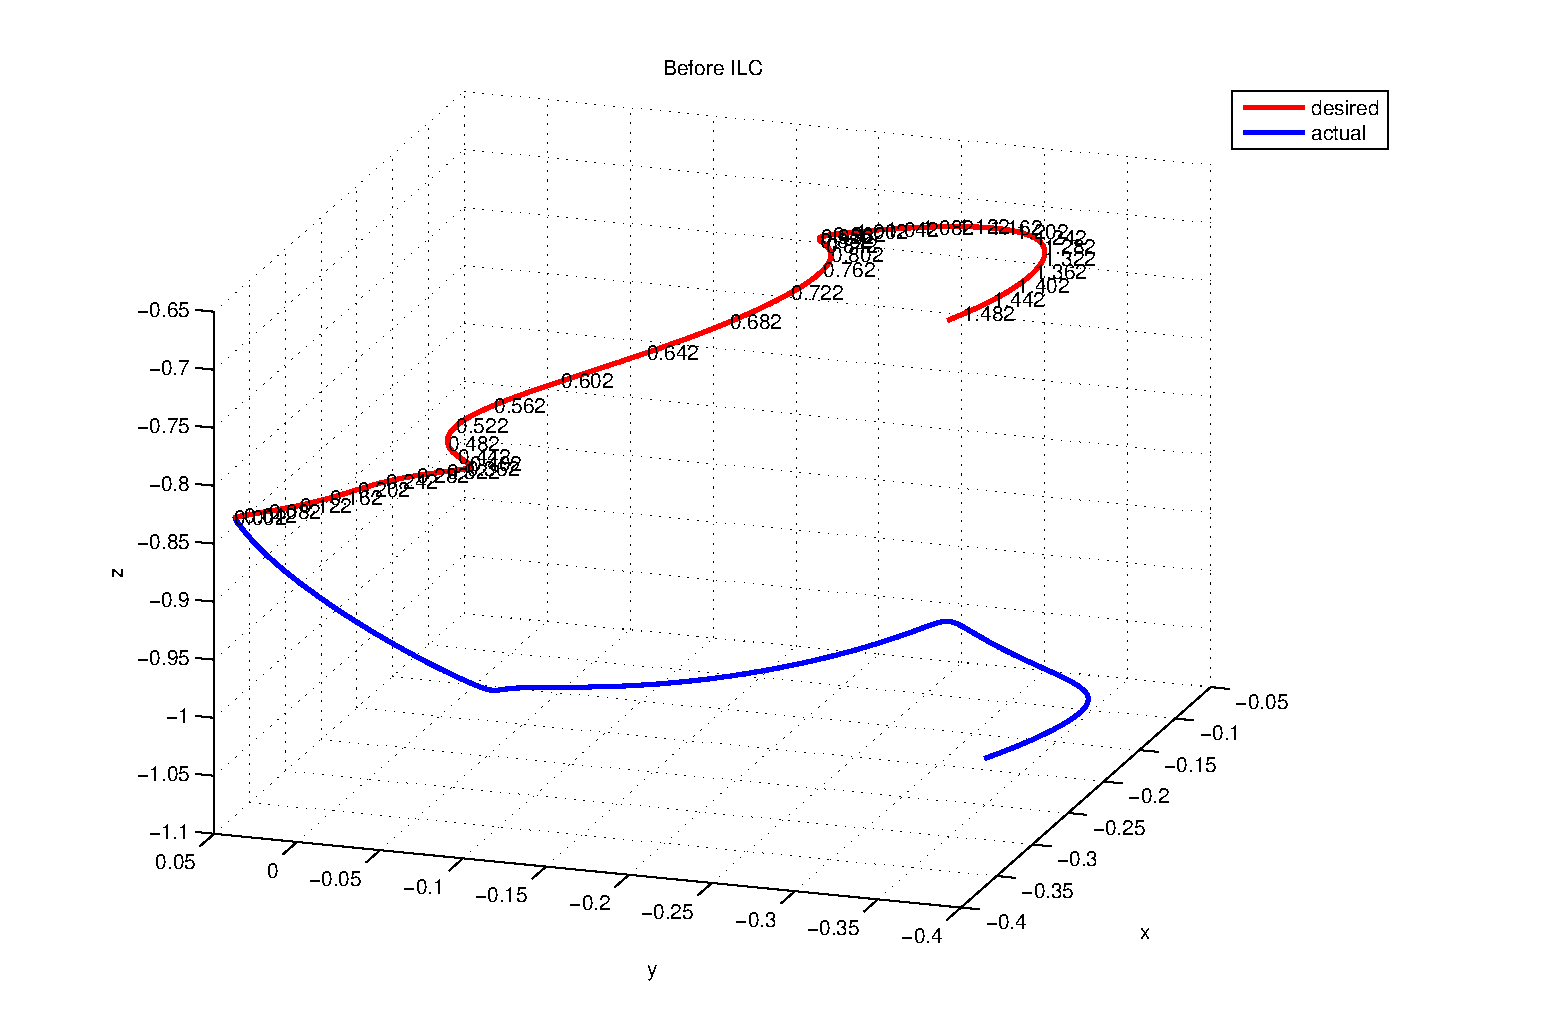
\includegraphics[width=\linewidth, height=0.15\textheight]{beforeILC.eps}
        \caption{(a)}
        \label{fig1}
    \end{minipage}%
    \begin{minipage}{.25\textwidth}
        \centering
        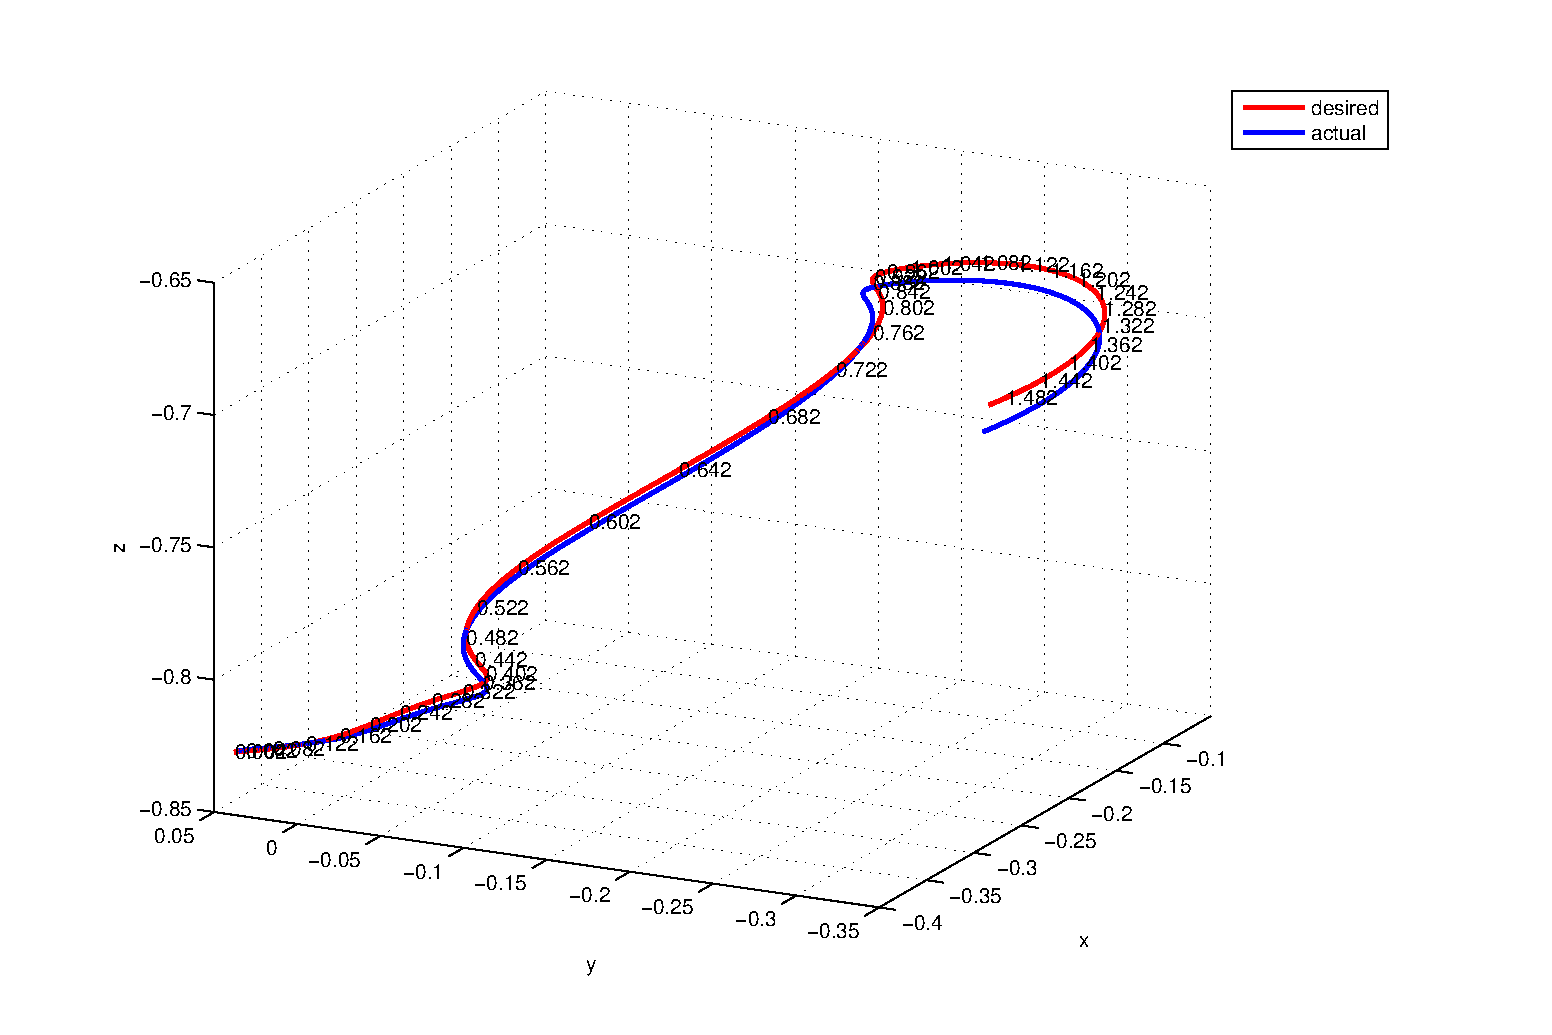
\includegraphics[width=\linewidth, height=0.15\textheight]{afterILCPseudoInv.eps}
        \caption{(b)}
        \label{fig2}
    \end{minipage}
    \begin{minipage}{.25\textwidth}
        \centering
        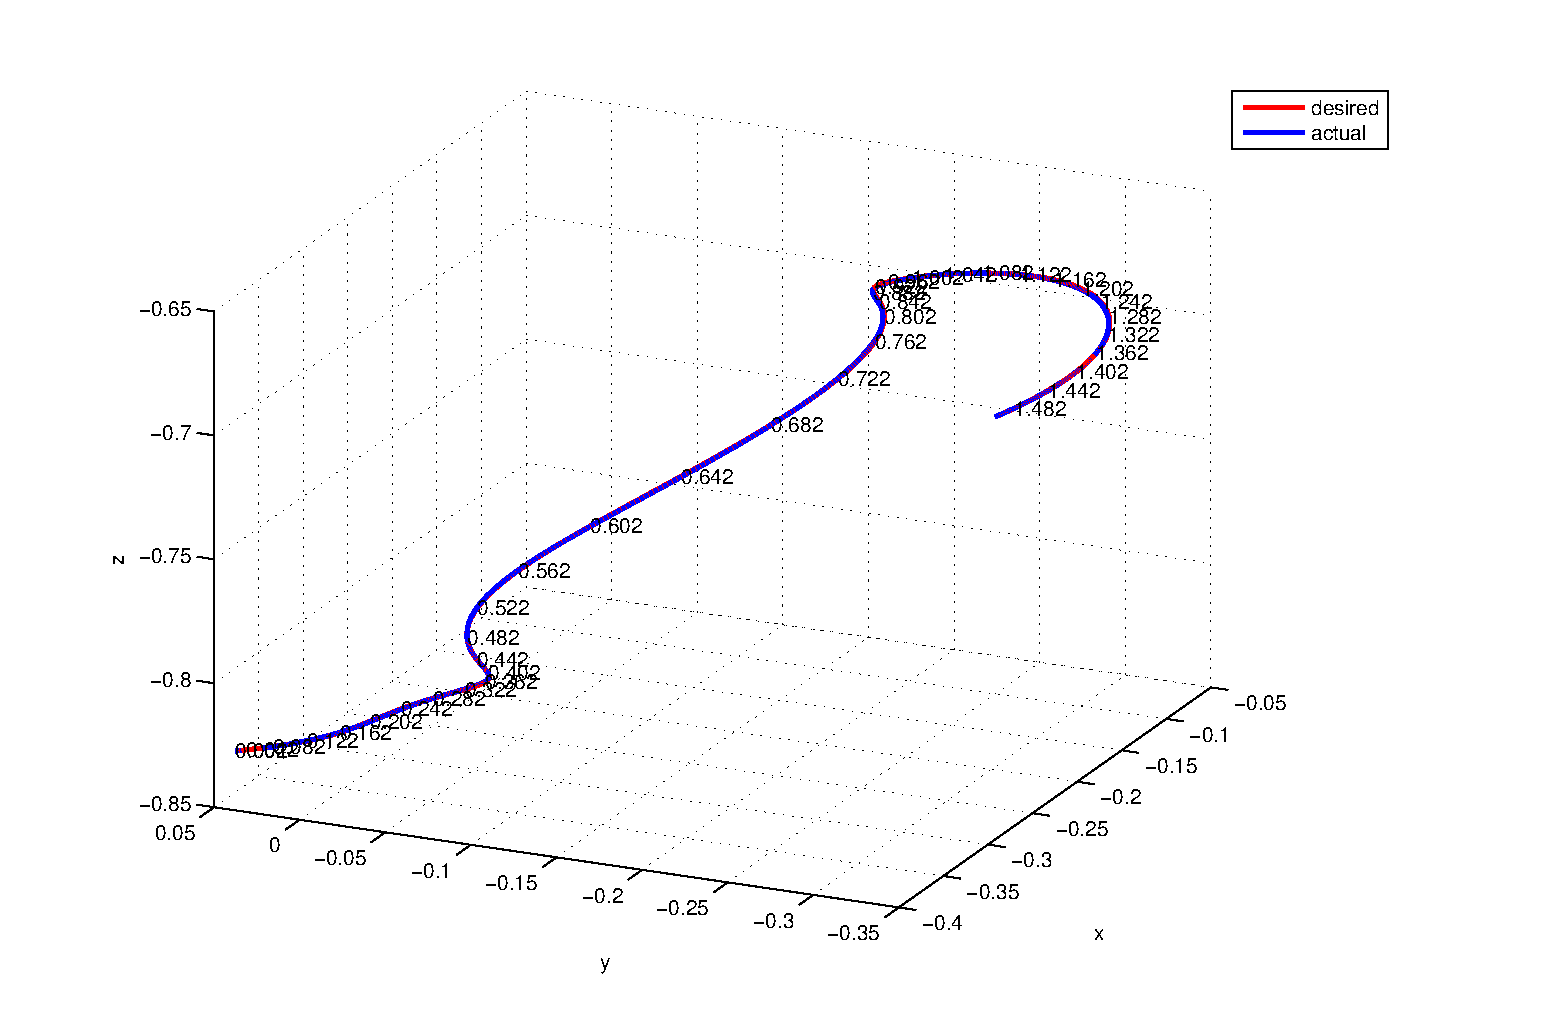
\includegraphics[width=\linewidth, height=0.15\textheight]{afterILCTLS.eps}
        \caption{(c)}
        \label{fig3}
    \end{minipage}
    \caption{Results showing the performance of trajectory tracking, before and after applying ILC (10 iterations). Reference trajectory is shown in red. Initially, in Figure~\ref{fig1}, tracking performance is poor. Final performances of pseudoinverse-based ILC and TLS-based ILC after learning are shown in Figures~\ref{fig2} and \ref{fig3} respectively. ILC with truncated pseudoinverse cannot approach the trajectory very well, and after 8 iterations starts to slowly diverge. ILC with truncated total least squares on the other hand approaches the trajectory very well, and shows excellent tracking performance that is also stable.}
\label{FigureILC}
\end{figure}

In the simulation results shown in Figure~\ref{FigureILC}, we consider a striking trajectory shown in red. Such ball-hitting trajectories in table tennis are generally composed of three parts: a preparatory phase, a hitting phase, and a relaxation phase. In the preparatory phase, the arm generally accelerates and picks up speed necessary to transfer the right momentum to the ball, intercepted in the hitting phase. The relaxation phase generally decelerates the arm and readies it for the next hitting task. 

ILC with pseudoinverse cannot approach trajectory very well, and after 8 iterations starts to slowly diverge. ILC with TLS on the other hand approaches the trajectory very well, and shows excellent tracking performance. For both methods, to be fair, we used the same truncation parameter, $\epsilon = 0.05$. This enables the pseudoinverse-based ILC to be more stable, i.e. without it ILC can show dangerous oscillations around some trajectories. However, even with truncation the pseudoinverse relies on the exactness of the model, whereas $\alg$ is inherently \emph{agnostic} to its accuracy. 

In practice we find that an additional adjustment in the form of \emph{current-iteration} ILC (\emph{CI-ILC}) 
%
\begin{equation}
\begin{aligned}
\sysInput_{k+1} &= \sysInput_k - \vec{K}_{LQR}\error_{k},\\
\end{aligned}
\label{fbILC}
\end{equation}
%
\noindent where we add the feedback from the previous iteration to the feedforward commands in the next iteration makes learning more robust. We add this current-iteration compensation to both methods in the results shown. 


\subsection{Applications in Robotic Table Tennis}

We performed the real robot experiments with a seven degree of freedom (DoF) torque-controlled custom made Barrett WAM arm capable of high speeds and accelerations.
\section{CONCLUSION}\label{end}

% shall we put inv. dynamics eq here?
The cost functional to be minimized considers the accelerations as the quantity to be minimized. It assumes that the feedback linearization of the robot is perfect, that is the inverse dynamics model for the robot is exact. Whenever the cancellation is imperfect due to inaccurate robot control, execution error will prevent the robot from achieving the desired trajectories. Execution errors will be considered in future work.

\bibliographystyle{plain}
%\bibliographystyle{./IEEEtran}
%\bibliography{./IEEEabrv,./iros2015Ref}
\bibliography{./humanoids2015Ref}

\end{document}
